\section{Trajectory planning} \label{sec:trajectory_planning}
\textbf{\textcolor{red}{IMPORTANT:}} to simulate the trajectory it is required that \href[]{https://petercorke.com/toolboxes/robotics-toolbox/}{\textcolor{blue}{Peter Corke's Robotics Toolbox}} is installed.\\

Usage:\\
\texttt{>> test\_trajectory('j', true)}\\
\texttt{>> test\_trajectory('t', true)}\\

\textbf{Problem:} to find a trajectory connecting initial and final points.\\
There are different methods for trajectory jeneration. Some of them are:
\begin{itemize}
    \item LSPB
    \item Polynomial (Qubic, Quintic)
\end{itemize}
In this section we will perform the trajectory planning of simple pick and place task using LSPB.
We used both joint space and task space trajectory planning as shown in Figure \ref{fig:trajectory_planning} below.
\begin{figure}[H]
    \centering
    \begin{tikzpicture}
        \coordinate (A) at (0,0,0);
        \coordinate (B) at (2,0,0);
        \coordinate (C) at (2,2,0);
        \coordinate (D) at (0,2,0);
        \coordinate (E) at (0,0,2);
        \coordinate (F) at (2,0,2);
        \coordinate (G) at (2,2,2);
        \coordinate (H) at (0,2,2);

        \draw (A) -- (B) -- (C) -- (D) -- cycle;
        \draw (E) -- (F) -- (G) -- (H) -- cycle;
        \draw (A) -- (E);
        \draw (B) -- (F);
        \draw (C) -- (G);
        \draw (D) -- (H);

        \coordinate (I) at (5,0,0);
        \coordinate (J) at (7,0,0);
        \coordinate (K) at (7,2,0);
        \coordinate (L) at (5,2,0);
        \coordinate (M) at (5,0,2);
        \coordinate (N) at (7,0,2);
        \coordinate (O) at (7,2,2);
        \coordinate (P) at (5,2,2);

        \draw (I) -- (J) -- (K) -- (L) -- cycle;
        \draw (M) -- (N) -- (O) -- (P) -- cycle;
        \draw (I) -- (M);
        \draw (J) -- (N);
        \draw (K) -- (O);
        \draw (L) -- (P);

        \node at (0.85,2.8,0) {$*$};
        \node at (5.85,2.8,0) {$*$};
        \node at (0.85,1,0) {$*$};
        \node at (5.85,1,0) {$*$};
        % home
        \node at (-2,7,0) {$*$};

        \draw[-,red] (0.85,2.8,0) -- (0.85,1,0);
        \draw[-,red] (5.85,1,0) -- (5.85,2.8,0);

        \draw[-,blue] (-2,7) to[out=0, in=90] (0.85,2.8, 0);
        \draw[-,blue] (-2,7) to[out=0, in=90] (5.85,2.8, 0);
        \draw[-,blue] (0.85,2.8,0) to[out=90, in=90] (5.85,2.8, 0);

        % Legend
        \node[left] at (-2.7,7) {Home};
        \draw[-,blue] (8,7) -- (9,7);
        \draw[-,red] (8,6.5) -- (9,6.5);

        \node[right] at (9,7) {Joint space};
        \node[right] at (9,6.5) {Task space};

    \end{tikzpicture}
    \caption{Trajectory planning}
    \label{fig:trajectory_planning}
\end{figure}
The task definition can easly be seen from Figure \ref{fig:trajectory_planning}. 
In the next sub-sections we are going to see the implementation of task space and joint space trajectory planning.

\subsection{Joint space trajectory planning using LSPB}
What is LSPB?\\
In short, Linear Segments with Parabolic Blends trajectory, is a symmetric trajectory with
trapezoidal shape of velocity profile, with constant velocity in central part of the path.
\begin{itemize}
    \item This type of trajectory is appropriate when a constant velocity is
             desired along a portion of the path.
    \item The LSPB trajectory is such that the velocity is initially ramped up
             to its desired value and then ramped down when it approaches the
              goal position.
    \item To achieve this we specify the desired trajectory in three parts.
    \item For $t\in\left[t_0 \quad t_b\right]$ and $t\in\left[t_f-t_b \quad t_f\right]$ the trajectory is described by a quadratic polynomial.
    \item For $t\in\left[t_b \quad t_f - t_b\right]$ a constant velocity, $v$, is taken.
    \item The blend time $t_b$ is chosen such that the position curve is symmetric.
\end{itemize}
The LSPB trajectory is defined by the following equation, assuming $t_0=0$:
\begin{equation} \label{eq:lspb}
    \begin{cases}
        \theta(t) = \theta_0 + \frac{\alpha}{2} t^2 & 0 \leq t \leq t_b \\
        \theta(t) = \frac{\theta_0+\theta_f-vt_f}{2} + vt_f & t_b < t \leq t_f - t_b \\
        \theta(t) = \theta_f - \frac{\alpha t_f^2}{2} + \alpha t_f - \frac{\alpha}{2}t^2 & t_f - t_b < t \leq t_f
    \end{cases}
\end{equation}

\subsubsection{Constraints of LSPB}
While driving Equation \ref{eq:lspb} it is assumed that $0 \le t_b \le \frac{t_f}{2}$, Other wise the trajectory can't be achieved. 
From this condition we can derive the following constraints:
\begin{equation} \label{eq:lspb_constraints}
    \begin{aligned}
        \frac{q_f-q_0}{v} < t_f \le \frac{2(q_f-q_0)}{v} \\
        \implies \frac{q_f-q_0}{t_f} < v \le \frac{2(q_f-q_0)}{t_f}
    \end{aligned}
\end{equation}
If $t_b = \frac{t_f}{2}$ then the trajectory reduces to mimimum time trajectory (Bang-Bang trajectory).
We have used equation \ref{eq:lspb} to define the trajectory in joint space and the result for sample trajectory between the following initial 
and final joint angles is shown in Figure \ref{fig:lspb_single} and \ref{fig:lspb_trajectory}.

For a single joint: $q_0 = 0\, and \, q_f = \pi$
\begin{figure}[H]
    \centering
    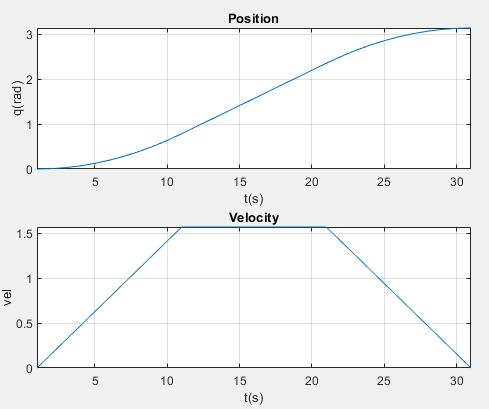
\includegraphics[width=0.5\textwidth]{images/lspb_single_joint.png}
    \caption{LSPB trajectory for a single joint}
    \label{fig:lspb_single}
\end{figure}
For all the joints:
\begin{equation*}
    \begin{aligned}
        \theta_0 &= \begin{bmatrix}
            0 & 0 & 0 & 0 & 0 & 0
        \end{bmatrix}\\
        \theta_f &= \begin{bmatrix}
            \pi & \pi/2 & \pi/4 & \pi/6 & \pi/8 & \pi/10
        \end{bmatrix}
    \end{aligned}
\end{equation*}

\begin{figure}[H]
    \centering
    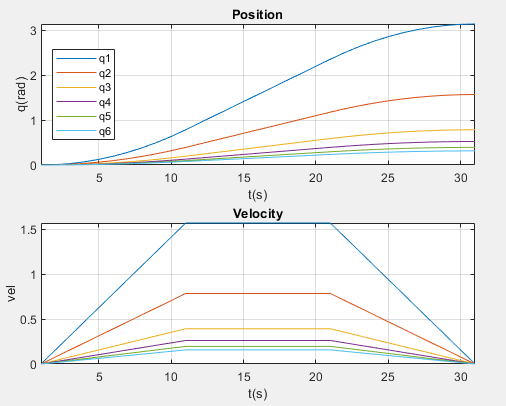
\includegraphics[width=0.5\textwidth]{images/lspb_trajectory.png}
    \caption{Synchronized LSPB trajectory}
    \label{fig:lspb_trajectory}
\end{figure}
For synchronizing the trajectories we have used the maximum $t_f$ of all the joints. 
This computation of time is implemented in the function $get\_time$.

\subsection{Task space trajectory planning}
For the task space trajectory planning we have followed the following steps:
\begin{itemize}
    \item Express the end-effector pose in terms of roll, pitch and yaw angles.
    \item Use linear interpolation to compute the trajectory for each of the roll, pitch and yaw angles 
          as well as the $X, Y, Z$ coordinates of the end effector (position).
    \item Convert each roll, pitch and yaw angles back to the rotation matrix.
    \item Generate the homogeneous transformation matrix using the rotation matrix and the position.
    \item Perform inverse kinematics to compute the joint angles for each of the homogeneous transformation matrix.
\end{itemize}
Note, if we don't generate enough points in the interpolation we can use LSPB to get more joint angles between each 
consequetive points.
The end-effector pose for straight line task space trajectory is shown in Figure \ref{fig:task_space_trajectory}.
\begin{figure}[H]
    \centering
    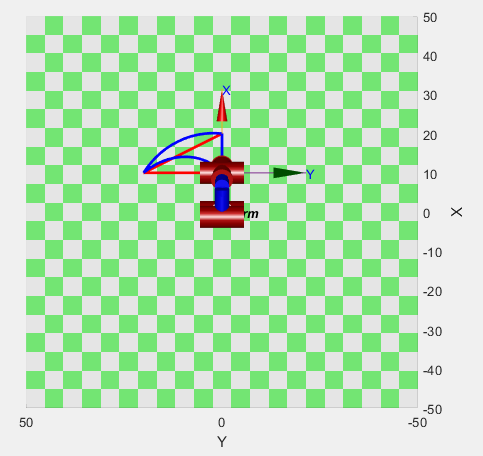
\includegraphics[width=0.6\textwidth, height=0.4\textheight]{images/task_space_trajectory.png}
    \caption{Task space Vs. Joint space trajectory, end-effector pose for triangular profile.}
    \label{fig:task_space_trajectory}
\end{figure}
Finally the pick and place task (contains both joint and task space trajectories) trajectory end-effector pose is shown in Figure \ref{fig:pick_and_place}.
\begin{figure}[H]
    \centering
    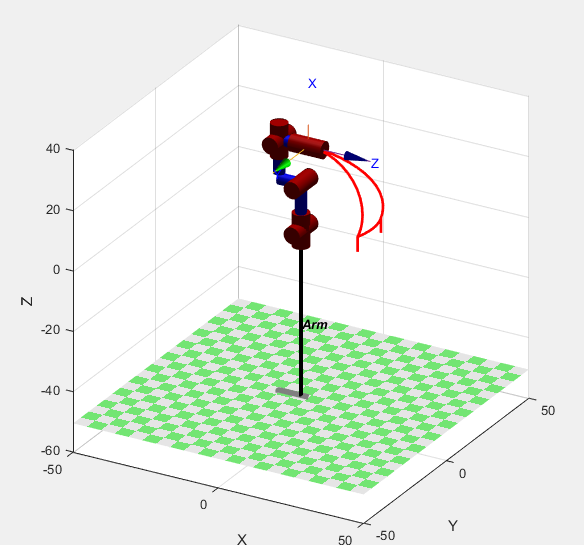
\includegraphics[width=0.5\textwidth]{images/pick_and_place_trajectory.png}
    \caption{Pick and place task}
    \label{fig:pick_and_place}
\end{figure}

